\documentclass[oneside]{book}
\usepackage{graphicx}
\newcommand\deletechapter[1]{}

\begin{document}

\begin{titlepage}

{
\center
\Huge
The Extra
\par
}

\vspace{.25in}
{
\center
\Large
By Samuel Alexander
\par
}

\vspace{-3.5in}

{
\center
\hspace{2in}
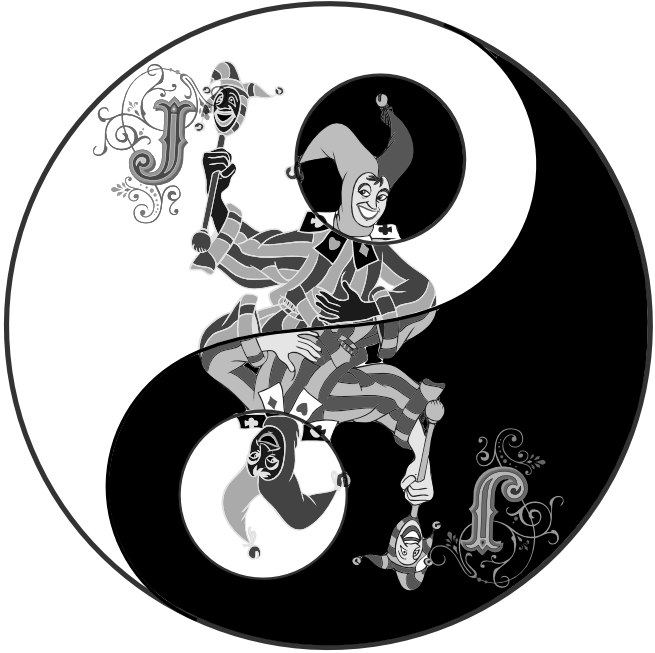
\includegraphics[width=600px,natwidth=840px,natheight=840px]{joker3.png}
\par
}

\vspace{.25in}
{
\center
``Would you rather be Zeus for a single day,
or see Zeus for the rest of your life,
only you can't tell anyone else you see him?''
\par
}

\end{titlepage}

\clearpage

\thispagestyle{empty}

{
\center

\includegraphics[width=300px]{slashdiv.eps}
\par
}

\vspace{.1in}

{
\center
\Huge
Part I
\par
}

\vspace{.25in}
{
\center

\includegraphics[width=300px]{yydiv.eps}
\par
}

\chapter{Prophecy}


``All arise!''  All were eyes as the judge assumed the bench.  The crowds took their seats as the stenographer
read out the time:  ``Twenty four words.''  Proceedings were in session.

The plaintiff was the National Library,
suing for possession of an unpublished novel titled ``The Extra'',
written by the late Franz Kafka, who starved before he could
finish it.  The defendant was one Eva Koffe, daughter of Kafka's secretary
at the time of his death.  Representing both sides in their absense was Max Brod,
the friendless lawyer whose love of interest outweighed
the conflict of interest.  Max Brod was such a mean lawyer,
he once evicted himself from his own house.

If Kafka had not been such a writer (the defense argued),
the Library would never have bothered to sue.
They would therefore base their defense on slandering ``The
Extra'' and its talentless hack of an author.  It was for this
reason the proceedings began with the
judge solemnly reading the book itself (organized
best as possible from the author's scattered scraps).

But before the judge could finish four paragraphs, a man in the audience stood up.
``Your honor,'' he announced uninvited, ``there must be some mistake, this book is
about me!''  ``Sit down!'' the judge ordered.  The man remained standing.  ``My name,''
he explained, ``is Joey Baloney.  Same as the character in that passage you read.
What's more, I match him perfect.  It must be some mistake I say again!''

``Who does this idiot think he is?!'' cried the defense's lawyer.
``Does he know how to behave in court?  Look at his outfit: talk about plain!
Why are these rifraff allowed in the city, much less in these halls?
Oh judge, make him sit down!''

``Get your butt in that seat,'' said the judge, unamused.  ``When you were born,
this author was dead.  I've heard of dying delusions, but we ain't in one.
It wouldn't make sense, there are computers and cellphones.
If your name is Baloney, it's purely coincidence.''   ``He's a liar,'' said Brod,
``you can't trust his name.''

``I agree with Brod,'' said the judge.  ``I know your type, Joseph, if that's really your name.
You rail against authority.  You would protest your own parents, if they had any power.
You're a lobbyist for people too lazy to pay you.
You know, Joey, when an unemployed man sees another man working, he thinks he's doing it
for money.  When an employed man sees himself working, he knows he's doing it for a cause.
Hippy!
If you had your way, you'd turn our policemen to dust.''


``I will not sit down,'' said the man in the stands.  ``I can prove what I say.
I can prove it three times!  In fact you've given me the fifth, because all those
things you just said about me, you only know it cuz you read it in that book.''

``Enough,'' said the judge, with a wave toward the sergeant.
``See the gentleman out.''  ``Wait, judge,'' said Baloney.  ``If you have me
arrested, they'll check my ID, there'll be a paper trail proving I am who I am.''

``He's right,'' said Max Brod.  ``Oh drag!  Let's ignore him.  His feet will
wear out.  Sergeant, see to it that Joey Baloney can't use the water fountains.''
(At this the judge giggled.)  ``It's a hot day; let him stand in a desert.''

A cacophany flooded through the hallowed halls.
All this talk about fountains made the audience thirsty,
but out of respect for the judge they refused to rise from their
seats.  One by one they scooted their chairs down side passages
to the court drinking troughs, and the sergeant at arms
checked every one to make sure it wasn't Joey Baloney.

\chapter{The Chairs}

The judge was reading from the manuscripts in a bored voice,
like a little boy in front of class.
%``The joker card represents villains because of its
%random, chaotic, unpredictable nature.
%``But imagine opening a
%deck and instead of finding a joker card, there's a dead rat: 
%weeks old,
%oozing with infection and crawling with maggots.
``That \emph{card} also represents a villain,
and that villain is Joey Baloney.''  
The judge frowned,
as if reminded of an overdue library book.

``Our chairs not good enough for you, then?''  He turned his glare toward
the Baloney in the stands.
``Sergeant, have we any better seats in these chambers?''

``No, your honor, they're the best we've got.''

``Well, the Senate's nearby, fetch some of theirs.''

The sergeant marched out of court and the judge leveled his gaze on Joey.
``Tell me again why you're standing, sir?''

``There's something amiss here,'' said Joey, ``that character in the book is me,
and that's quite impossible if it was really written by that author.
Even if you overlook the temporal impossibility---I was born after he
died---there's the fact I never gave permission to use my likeness.''

``Well why didn't you say so?'' said the judge.  ``That's a very reasonable
complaint, we'll address it straight away!  Come, take a seat in the front,
your issue is our highest concern.''  The judge even went so far as to pat the
seat of an empty chair beside him, a duplicate of his own.

Joey was too smart for that trap.  ``I ain't falling for your tricks,''
he said, ``I'll stand til my complaint is addressed.''

The judge was outraged.  He'd have sentenced Joey to the electric chair,
but he was afraid of a papertrail proving his name.
``You're worse than Hitler's evil twin,''
he said, ``you're worse than Genghis Khan in a thong!''  He was going to shout some
other mean things, when the sergeant returned to the courtroom.

``Here your honor, one of the best seats they got.  Seat of the Senate majority
leader.''  It was a giant seat, emblazoned with seals and surrounded by
desks and podiums, lesser seats for lesser senators.

``I will not sit,'' Joey said, turning his nose up at the furnishings.

``Alright, go get something better,'' said the judge.  The sergeant left again.
For a second, the judge wished he had a `Fasten Seatbelts' button.
Or failing that, a sudden burst of turbulence.
Or failing that, an iceberg.  Would Joey sit on a lifeboat seat?

The judge tilted his seat back, plopped his feet on the podium, stretched
his legs luxuriously.
%It was clearly an attempt to seduce Joey into sitting.
He kicked off his shoes to get more comfy, his socks were speckled with mud.
But Joey wasn't seduced, and Joey still stood standing.

The sergeant returned an hour later with a twisted silver chair, cold
to touch.  It hissed and slithered
like the beams were snakes.  Carved in back was a
hammer-and-sickle crossed-out with an X.  ``Hard to beat this one,'' said Sarge,
``the chair of no less man than Senator McCarthy!''

``Won't sit, won't sit!'' Joey stuck out his tongue.

``Sergeant, stop playing around!'' cried the judge.
``What other chairs did you find there?''

``Let's see,'' the sergeant started counting his fingers.
``There was a chair made of fractals, a chair of rubber ice.  A chair made of words,
but it was copyrighted.  There was a chair forged in Vietnam, many veterans died
to do it.  There was a water-chair, like a waterbed in chair form.
A chair carved out from one huge diamond.
There was a chair made of hair, but it needed a haircut.
Chaircut?
There was an astronaut's chair, but it was upside-down.
There was a rocking chair sat in by the Beatles.''

``None of those will do,'' said the judge.  ``Don't come back til you've
found the finest chair in the Senate!''  The judge was almost ready to
order a seat assembled around Joey where he stood.
%craftsmen to assemble a seat around Joey where he stood.

At long length the sergeant returned.  He bore the chair Barack Obama
sat in before ascending on high.  It was crusted with gems and opals, some
big enough to be decked with smaller jewels.  It was draped in purple silk.
% of Persia, shimmering with an aura of priceless perfumes.

``Dear sir,'' said judge to Joey, ``this throne is yours, please accept your
coronation.  All you've got to do is sit in it!''

But Joey would not sit, even in that golden throne.
In despair, the judge had it melted down for scrap.

\chapter{The Drink}


A dozen witnesses had come, ignoring Joey Baloney like a statue.
%(Several had been famous celebrities.  No relation
%to the suit, but the judge considered
%meeting celebrities a perk of the bench.)
The judge needed a break.  He declared a long recess.  Together with his lawyer,
stenographer, and sergeant at arms, he walked out of the chambers.
They reappeared through a little window looking out
on the playground.
%The judge began playing on the swingset.  Brod and the stenographer
%jumped on the see-saw, and the sergeant at arms went for the monkeybars.

Joey was thirsty, but gave no sign of wavering.
%To pass the time, he took a violin from his luggage and played awhile,
%a song mixing melancholy with joy.

In front of him there sat a young beauty.  If Joey was in a desert,
her beauty was his oasis.
She was almost perfect.  The only flaw was she'd slept wrong and a
strand of hair stood up awkwardly.
She was so lovely, a gentleman once gave her a gift of goldfish heels:
with little fish swimming `round in the heels, they were the world's
most impractical shoes.

She turned in her seat and smiled.  ``I'm on your side,''
she offered.  ``I can't believe the injustice you're suffering.  The punishments the
judge has heaped on you.  What awful and lowly things the lawyers have said about you all day.''

``If I'm an awful and lowly man,'' Joey said, ``it's because I've stepped on the toes of giants.
I'm not resentful.''

``The defense attacked you so viciously,'' she said.  ``And you're innocent.
You're only trying to defend your likeness.  You're doing them a favor letting them know
something's wrong.''

``I am not resentful,'' Joey said.  ``I'm happy about it, it gave me the chance
to meet you.  What's your number?''
It was a little forward of him to say that, but
Joey always believed that in a land where love is
forbidden, you have to smuggle it in.

The young lady giggled, fingers playing with her hair.  A golden ring glinted in
the light.  ``My phone isn't on me, sir!
I do like you though.  I'm not just saying it to avoid exchanging digits.''

``I'd give you mine,'' Joey said, ``but the judge would say it's copyrighted.''

His partner smiled, offered her hand.  ``You're funny, Joey.  It's alright if I call you that?
Is Joseph better?''

``Joey is best,'' said Joey, alchemying the handshake into something tender.

``Joey is best,'' she repeated.  Then she laughed.
Joey broke the handshake moments before she herself was going to.
``Talking with you makes me happy,'' she said,
``there's something playful about you.''

``Playfulness is in my genes,'' Joey said.

``I can't believe I'm saying this,'' she said, ``but you make the hairs stand up on
my arms.''

``Stand with me, we'll defy these tyrants together,'' offered Joey.

``I'm not as bold as you sir.  The only reason you're outside bars
is they're scared of proving your name.  My own is unimportant, they'd throw me in
jail for the both of us.''

``Stand by me, we'll live happily ever after,'' Joey haggled.

``Let's sit down together!'' she said.
Then in a suggestive register, ``I'll sit on your lap.''

Now Joey understood all.
%, and he knew the cruelty of his enemies.
``Off, whore!''  His demeanor changed.  ``I see what you are.
The court prostitute!  How much is the judge paying to sit me down?''

Tears welled in her eyes.
She liked Joey (he had a resemblance to her father, and it was growing stronger).
If he'd put her on his lap,
she'd have given him everything, would have sworn
her heart and soul to him, right hand on the bible.
Instead he held her in contempt.
His judgment crushed her like a death sentence.
She appealed with her eyes, but found no leniency.

``Then, I'll give you a present, for what might have been.''
She cupped her hands, she caught her tears, she lifted them toward him
from her seat.  Joey paused, caution versus thirst.
Caution down, he took her cupped fingers to his lips.
He drank up her tears.  They were delicious.  He swallowed and his thirst was cured.
%With leftover sobs, she
%leaned down (a difficult proposition from her position)
%and lovingly washed Joey's feet.

When no more tears would come, the maiden fled.
Out of respect for the judge, she crawled out on all fours.
%rather than stand up in his courts.




\deletechapter{

\chapter{The Foodfight}

A dozen witnesses had come by, ignoring Joey Baloney like a statue, and now the
judge needed a break.  He declared a short recess for lunch.  Together with the lawyer,
the stenographer, and the sergeant at arms, he walked out of the chambers.
A minute later, the four of them appeared through the little window that looked out
on the recess playground.  The judge began playing on the swingset.  Max and Franz
jumped onto the see-saw, and the sergeant at arms went for the monkeybars.

Inside the courthouse, the rustle of lunchbags was gradually drowned by a
growing murmer.  Spectators were arguing whether or not Joey Baloney really was the
same Joey Baloney from Kafka's unpublished novel.  They started forming little cliques,
and then little cliques swore alliances and turned into bigger cliques, and the volume
of the shouting grew.  Joey himself was the only man not arguing.

``Is that what you think?  Then why don't you take that egg and throw it at me?''
A handsome young man in a junior officer's service dress taunted a superior officer.
``Egg?'' came the retort, ``You can't handle egg!''  And then the egg flew threw the air.
This sparked a chain reaction and in moments, the entire courtroom was alive with
flying vegetables.

A piece of spiced tomato barely missed Atticus Finch's face.  Solemnly and with tremendous
patience, Atticus opened his shiny briefcase, took out a rifle, and loaded it with
garbanzo beans.  With steady, careful hands, like a surgeon, he took aim at his slavering enemy.
He pulled the trigger; suddenly his enemy was felled, chest splattered with chickpeas,
mouth frothing.

``Confound your logic!'' bellowed a famous prosecutor, throwing a handful of rice as if to
blind the opposing side.  ``I happen to know, from the head of a nursing home, this man who
calls himself Baloney didn't even cry at his own mother's funeral.  Is that a man you can
trust?''  He was silenced by a coldcut sandwich to the mouth.






(The court goes on lunchbreak (the court officials withdraw).  The audience starts fighting
over whether or not Joey is right.  This degenerates into a foodfight.  It turns out everyone
from the audience \emph{except} Joey is an important character from various fictional
court scenes.)
}

\chapter{The Stenographer}


``Did Kafka get his ideas by digging in graves?''

The defense attorney was deep in the throes of slandering the
deceased.  He was skipping about,
dancing and singing the words.
``Kafka said he was Dostoevsky's blood brother.
If that's the case then who was the father?''

``Maybe they were half-brothers,'' the judge giggled.  ``A Russian and a German,
\emph{someone} was digging around!''  This drew childish laughter from the
audience, which pleased the judge tremendously.  Joey Baloney stood, refusing to
break his solemn filibuster.

``You're right, judge,'' laughed Brod.  ``Could explain where 'evsky got
%the idea for
Smerdyakov.  I always thought he looked the part.''

``If that's the case,'' chortled Judge, ``Kafka should've hanged himself.  Preferably
before writing this retarded book!''

``Next, your honor, I call the court's attention to Kafka's name.
What kind of name is Kafka?  It sounds like
something you'd buy at Starbucks.  `A
Kafka-latte.{'}''

``Objection,'' said the court stenographer.
%  Everyone turned toward the quiet source.
%It was the court stenographer.

``Explain yourself!'' said the judge.  He wasn't used to objections in his court.

``Well,'' said the stenographer, ``I feel rather silly bringing it up, you know,
but I'd rather the kind Mr.~Esquire wouldn't bash Kafka's name.''

``Why not?!'' asked Brod, casting a hateful look on the poor typist as if it were Joey Baloney
himself.

``The thing is,'' said the stenographer, ``it's my name too.  Just a coincidence,
I assure you, no relation to the author.  I just don't think it's considerate
of you.  Maybe someone in the audience is named Kafka too.''

``Is there a Kafka on board?'' boomed the judge.
%, pointing his gavel at the great washed masses.
``Maybe you, mischief-maker?'' He looked now at Joey, as if Joey was an unwelcome bill at a restaurant.
``Still standing, are you?  How impolite I've been to my guest.  Have a seat, have a seat!  My wife will bring you snacks and
a beer.  Maybe you'd like a table to put your feet on?  Care to watch the telly?''

``No Kafkas today, sir,'' piped the sergeant at arms.  ``I'd know, sir, they're all regulars.
All but him I mean,'' with a nod at Baloney.

``Say, stenog,'' began the judge, ``Joey Baloney says he's in `The Extra'.  Does the manuscript
say how to make that character sit the hell down?''

``I wouldn't know, Judge.  I haven't read a lot of Kafka.  Actually nothing but the Metamorphoses, sir,
and that was ninth grade, sir.  You know they keep me too busy to read, sir.  I'm here doing my one-year
duty to pay off writing school debts, they don't give me a moment's rest, sir.''

``Don't like your job then?'' asked the judge.

``Not exactly sir,'' said the stenographer.
``I always thought I'd like writing, I wanted to be a great author, but now I'm doing it,
it's not for me.  All day I write down these bureaucratic proceedings.  Word after word.
Sometimes I ask myself: how many words 'til a man can be free?
To be honest sir, I only
come in any more to put bread on the table.  (My father calls it a \emph{Brodberuf}; that's
German, sir, for \emph{bread job}.)
So when the kind lawyer makes fun of my name, sir, it's insult added to
injury, sir.''

The stenographer didn't know how true `insult added to injury' was.
Believe it or not, there already was a great author in the room, but it
was the judge.  The previous stenographer had
done all the work.  He'd writ a great story and published anonymously,
with a cypher to prove his name later.  When he saw how popular his
story'd got, he gave the judge two
weeks' notice, told him he was author of the famous book, and showed him the
keys to prove it.  The judge stole the keys and stole the credit, and the
former stenographer died poor and obscure.

``Man, I'm sorry, I had no idea,'' Brod apologized.  He crossed the floor and embraced the stenographer,
showing his sincerity.


``And it especially hurts,'' the stenographer went on through the embrace, voice cracking a little.
``Because recently I want nothing more
than to be a lawyer like you, Max.  The truth is, I have a great admiration
for you, you've even inspired me to study law in my free time.''
Brod was genuinely touched.  It was a rare bonding moment, and the audience (all but Joey)
were moved.  Court historians would look back
for decades to come: the year Max Brod made his first friend.

Of course, the problem with being both a writer and a lawyer is that no-one can
understand all of your work.

As for Max, he was so moved he indulged in a fantasy.
He imagined they could all start a rockband.
The stenographer would play keyboard, of course.
The sergeant, with his wicked rifle, would make a great guitarist.
The lawyer would do lyrics, rapping about right and wrong,
and the judge would be on drums, banging with his gavel and rubber stamp.

The stenographer went on.  ``I hate to toot my own flute, but I've gained enough
lawyer's intuition I could say a thing or three about this Baloney case.''

``You don't speak much,'' the judge said.  ``But when you do it's
insightful.  Tell us about Baloney.''

The stenographer sized Joey up and down.  It took longer
than usual, there was more `up and down' to Joey than his seated peers.
``Well sir, contempt me if I'm wrong.  This man's the worst kind of anarchist.
Eats granola bars and protests polar bears.  He's an awful hipster, sir.
He's a communist sympathizer, but put him on the wall's other side and he'd sympathize
capitalist.  He---''

He was cut short by the judge's laughter.  ``You rascally little devil!'' the judge
declared.  ``Sergeant!  See to it the stenographer gets a \$20 bonus!''

``Thank you sir, but I don't know what you mean,'' said the typist.

``Don't know what I mean!''  The judge slapped his knees with the gavel.  ``You've read \emph{The Extra},
you've read it three times!''


\chapter{The Policeman}


The judge looked upon the rotting manuscripts, and drew his eyes away.
He looked upon the rotting court, and there stood Joey Baloney.

The next expert witness was Chief of Police.  The defense wanted his opinion on a certain
joke in ``The Extra''.  The assumption was that by getting the police to ridicule the work,
it would be slandered in the eyes of patriots.  As he entered, the Chief
shot a glare at the sergeant at arms, they were bitter rivals.

``Good afternoon chief, so glad you could make it,'' said Brod.

``Glad to be here, Brod,'' said the chief.

``You know, Clete,'' the judge said to the chief,
``I can't help but wish we didn't have to spend
all our time on garbage like this book here.''

``Come on, now, we don't have it that bad,'' said the chief.
``You should hear what my brother has to deal with.
There's an ancient Greek baby named Cryossus (his name is a joke
on Colossus, but has since been taken into everyday language with
solemn and dignified meaning).  Somehow some fingerpaintings of his
have survived to the present day, and there are these academics
just devoting their whole lives to studying them!  But they're just
fingerpaintings from when he was less than one year old, and
nothing else is known about the man himself.''

Brod cleared his throat loudly.
``I understand you wanted to hear my opinion on a certain
piece of some book?'', said chief.

``That's right,'' said Brod, ``but first I believe you had something to tell us about jokes in general?''

``Oh right!'' said the officer, remembering his coaching.  ``Listen judge.  You can't trust jokes.
They're like mafia fronts.  The mafia runs all these stores, and they sell you good stuff, but the goods aren't
the purpose.  There's sinister things done behind those stores.  It doesn't even matter if they
sell you anything at all.  Same thing with jokes.  Authors use them to hide things.  So it doesn't even matter
if the joke makes you laugh.  It doesn't even matter if it's funny.  There's sinister things done behind it,
and that's the joke's purpose.''

``Thanks,'' said the judge, ``I'll keep it in mind.''

``Now, chief,'' Brod directed, ``This unpublished book contains the following joke.  Tell us if it should
see the light of daylight.''

\vspace{2mm}
\noindent \textit{The Joke}
\vspace{2mm}

Knock knock.  The apartment's got couches, but the intruder ain't here to sit.

It's a policeman.  He's thin, in the bad way.
Tall like a stick.  Looks unhappy to be there.  Miserable, even.  You can tell he'd
rather be anywhere in all the world than at this apartment.  He'd pay any price to just
get away.

``Sir,'' he says, ``We've received a complaint from your wife, says you're not having enough fun.''

Just then there's a crash down the hall.  The policeman's wife has arrived.  She's ugly and mean: who would
ever marry her?  She's berating the poor cop, shouting at him for harassing the poor man, for being
such a wet blanket.

\[*\mbox{ }*\mbox{ }*\]

``Stop!'' cried the chief, boiling with rage.
``Never have I heard such damnable garbage.
I've heard quite enough!  This Kafka fellow, why, he just ain't American.''

He spun toward the stenographer and suddenly demanded:  ``How much longer
is the stupid thing anyway?''  Caught off guard, the stenographer was
struck dumb.

An idea occurred to the chief.
``Yo, judge, here's what you should do.  Make this damned \emph{Extra} be the Book
of Jafar.''

``The Book of Jafar?'' asked the judge, eyebrow raised.

``You don't know it?'' said Chief.  ``Oh, you'll like it, I'm sure!
Once upon a time, there was a wizard named Jafar.
Jafar was great, every book he wrote sold wide.
Jafar got fed up.  He hated that fame.  Used all his
arts, and used all his powers, and crafted a magical book of obscurity.
A book enchanted with spells so that no-one would read it, or even know
it existed.  And you know what?  It worked.''

There was a crash in the hall.  The police chief's wife had arrived.
The stenographer finally recovered and answered the question:
``The chapter's unfinished.''

\clearpage

``You know,'' said the judge to the stenographer.
``You have to be careful as a writer.
There once was a writer who died just as he wrote
the last verse of a poem on paper.  Nobody knew his password,
so the beginning verses were lost.  It became an example
of a great poem with an end but no beginning.''

The stenographer reflected on the judge's words.
It occurred to him that the way the chapter went on after
appearing unfinished was an example of a literary
optical illusion.  The stupid sergeant at arms merely
wondered why anyone would write a poem about paper.

\chapter{Intermission}


Many words had been exchanged in the court, and it was late.
Or maybe early: hard to say without studying the
transcripts.  Around the bleachers, jurists slept in their seats.
Some had brought sleeping bags, and were
sprawled out in the aisles, but no-one dared stand, no-one but
Joey.  An amorous purr drifted from somewhere in back of the
hall.  Joey yawned and rubbed
his eyes.

An old man on the balcony was eating a bag of
chips, and his crumbs flittered into the stands.
Crusty particles burned Joey's eyes and he
nodded off, dozing on his feet.

In an uneasy nap the words of the court were mixed up and
scrambled, and Joey dreamt two dreams, interdependent opposites
woven like a rope of snakes.

\vspace{2mm}
\noindent \textit{Joey's Two Dreams}
\vspace{2mm}

I was right in the middle of my speech.
``The joker card represents villains because of its
random, chaotic, unpredictable nature.  But imagine opening a
deck and instead of finding a joker card, there's a dead rat:
weeks old,
oozing with infection and crawling with maggots.  That \emph{card} also represents a villain,
and that villain is Joey Baloney.
I met him in a glass elevator, the only other occupants were a little boy and his mother.
Joey whipped it out of his pants and began pissing in the corner.  He was raving like a lunatic,
informing the boy, in quick and feverish narratives, where babies come from.''

Among my audience I saw worried glances and confusion.  I'd been invited to this renowned conference
to present my research.  And here I was, telling them about Joey Baloney.
Instead of sterile academia, I was unveiling a grander truth, forbidden,
the world was not ready for it.
A speech that would see me in jail or dead by night's end.

``Joey Baloney's words rushed out in breathless rapidity, he was struggling to tell the
boy everything he could about human reproduction before I could stop him.
I was a policeman back then.  Used to dealing with crazies on the elevators,
but nothing like Baloney.
I stood gaping for a few seconds.  Precious time for Joey Baloney to continue his shpiel.''

I saw the looks turning to panic.  Famous gatekeepers of knowledge wondering if I'd lost my
marbles.  I'd have to hurry if I were to deliver this truth before the front row would
rush and tackle me.

``The mother shrieked for help.  My ears rang, with trembling hands I leveled the tazer, I fired.
Joey Baloney fell to the ground, lay in his own steaming urine, and yet his monologue continued!''

Women were fainting now in the audience, cries of panic in the back.
Colleagues were rushing to them, make room make room!, pleas falling on deaf ears
as distinguished professors sat transfixed.
The first to rush me was a war veteran, a Harvard dean who'd
killed twenty Germans with his bare hands.
He stumbled, fell.

``The boy was sobbing, unprepared for the vulgar knowledge.
I threw the tazer aside, grabbed my firearm, whipped it out of my pants,
shot Baloney in the head!  The elevator shattered.''

I shouted into the mic to subdue the rising protests.
Career suicide, that's for sure, but more than that, it was real suicide.
There are truths which must not be spoken to those who do not know them.
Truths that shatter innocence, that complicate the carefree world.
I know things that'd make your mother cover your ears.
Things so astounding they'd put me to death.
And here I was, shouting them: to a man like me, truth
is more important than breath.
A giant in the world of womens' studies threw herself at me.
I brandished the mic, I thrust it into her crotch, I stamped on her toes.
Don't stop me now!

``Joey Baloney has gone by many names.  Genghis Khan; Hitler.''
I kicked a Fields medalist as he lunged for the mic.  Our fathers
died for freedom, a few ivory towerists can take a kick for truth.
You see, some truths are so forbidden, even if you want to tell them
you can't.  You have to tell something else instead, something silly or obvious or both,
a stand-in.  Those in the know will understand.
Sign of solidarity, reinforce the besieged truth.

``The ancients referred to him as Loki, great trickster.''
I ducked just in time to dodge the first hail of bullets.
Amazing how the authorities rush when the status quo is
really threatened.
``He's the type who invents new kinds of crimes just for the novelty.
Like take someone else's writing, pass it off as his own, and make
it public domain, just to cause trouble.''
%He'd take this very speech itself, and say: This work is
%released into the public domain.  Even though it's certainly
%not!'' 

A dozen SWAT commandos tackled the podium.
An assault rifle blasted my brains all over the conference hall.
And yet with labored breaths I went on.
%(It's funny, I felt no pain, only thirst.)
Only the riot police heard me any more, but that's alright,
because you hear me, and you will hear me to the end, even if your mother
doesn't want you to.  No-one will deny you this fruit of the tree.
``I was unconscious briefly after we fell from the elevator.
When I came to, Joey Baloney was whispering to the boy with labored breaths,
though only I could hear him anymore.''
%I wasn't dead, because no-one knows what's after death.
%By which I mean, the unknownness is part of the \emph{definition},
%not just a side effect.  The first man whose afterlife we know about, will never die because we'll
%remember him eternally.  The point is, I do know what comes after, though that's not the
%knowledge I mentioned earlier, it's just a footnote in fact.

``For years, people would imitate Joey Baloney, exposing themselves to children
and shouting unwelcome biology.  Like Joey, they'd always introduce themselves:
Ladies and Gentlemen, Joey Baloney!  It got so bad the government built
hemlock drones to shoot whoever said that phrase.''

``But after time, thanks to the drones, people forgot what was even supposed to come
after the Ladies and Gentlemen, Joey Baloney.  It was a conundrum, the
whole point was to stop the transmission of that forbidden knowledge,
now that no-one remembered it, was it still legal for the drones to shoot them?
In the end it became a crime punishable by death to even imagine what Joey
said after his introduction.
But what the imposters were supposed to say, what Joey Baloney said after his
introduction, went like this\ldots''

I'm too weak to speak aloud now, no time to finish.
No time to present my proof that Joey was there at the start:
He whipped a rib out of Adam's pants, he stuck it in Eve, and that's where
babies come from.  The important thing is, I know.
Remember that if you know nothing else about me: I know.
%, if you know nothing about what happens
%to me after my death: I know.

``A hush came over the conference as the speaker lay in his own steaming blood.
By sheer force of habit, the organizer picked up the microphone and uttered the
outro.''  Ladies and Gentlemen, Joey Baloney.


\chapter{The Judge's Speech}


``How many words will it take, before our policemen turn to dust?''

The judge was infinitely exasperated at Joey Baloney's stand,
charging his speech with feeling.
%Bloodless fingers clutched the podium.

``How many words will it take before old men bow down to the wisdom
of boys?
%How many words until joy replaces terror in the hearts of the world?''
How many words until schools let out early, and teachers make a decent wage?
How many words `til lambs lie down with lions?''


%As he spoke, the judge's words seemed to project lofty images in the hearts of the court,
%sprawling panoramas of human nature and all its faults.
``How many words will it take
before unemployment protestors are laid off?
How many words until the meek demand their inheritance?
How many sentences must this court deliver before this court's sentences are obsolete?''

``How many words will it take, til every dissenter assents?  How many words will it take,
to replace warfare with wars of words?  Fold swords into pens?
How many words til green fields and rivers
blossom in Death Valley?
How many words will it take `til
colonies are uprooted and native kings restored?  `Til pharmacies are replaced
by shamans?  `Til propaganda is dragged through the mud?  How many words will it take?''

``How many words, Joey, if that is your name, until capitalists pay for their greed?
%How many words must this court spend before mankind lives as one?
How many words must you steal from this court,
Joey, before man stops stealing from man?  How many words must the courts print before
the chains of copyright come off?  How many words til cars turn into bikes
and soldiers return home?''

Elder statesmen wept and young activists trembled.
``How many words must this battle go on?
How many words will it take to satisfy people who demand to be offended?  How many Kumbaya's
`til every Baptist is Buddhist, `til Muslims join Womens' Lib?
How many words must we trade before stock markets turn to farmers
markets?
How many words before the weapons that end wars will end?''

A tear gathered in the corner of the judge's eye, growing until the gravity of
his words loosed it.
It caught a holy ray of light in its fall,
bending every lawyer in the court to weep openly.
Every woman covered her face.
And still the judge's speech went on, the light in his eye blinding every clerk.

``How many words til civil wars become civilized? 
How many words til history's wrongs are righted and its rights distributed equally?
How many words until high school students read willingly, 
and Satan ceases his ceaseless sieges on God?''

The courthouse shook.
The universe paused its weary
acceleration, a moment of respectful silence in the cosmic background radiation.
The judge lifted his gavel, he pounded the dais,
damn the protocols, use it just for emphasis.  The gavel's head broke off,
the judge tossed the handle and raised a fist to heaven.
``How many words, `til our policemen turn to dust?''

Joey sat.

\clearpage

\thispagestyle{empty}

{
\center

\includegraphics[width=300px]{yydiv.eps}
\par
}

\vspace{.1in}

{
\center
\Huge
Part II
\par
}

\vspace{.25in}
{
\center

\includegraphics[width=300px]{slashdiv.eps}
\par
}


\chapter{His Royal Judgesty}


The judge's apartment was cramped and dirty.
It was the very smallest apartment in the whole city limits.
You couldn't open the door full way, because it would hit
the foot of the bunkbed, so instead you'd have to squeeze in
sideways, pulling your groceries behind you.
A gallon of milk wouldn't fit through, you'd have
to buy halves.

The judge slept on topbunk, his wife underneath.
The bed was too short, the judge's feet would touch
the door if he stretched out his legs.
A chandelier with very sharp claws took up the rest
of the overhead.  It had ripped up many a suit.
Portable cookware and dishes, fit for a campground,
were scattered around the floor.
Boxes of cereal and half-used spaghetti stuck out
from under the mattresses.  At least there was
a garbage disposal, so the judge could throw away keys.

``You're an idiot!'' the landlord had cackled as soon as the lease was signed.
``A sucker born every word!  Take the place, and every
lawsuit it comes with!''

But it wasn't that slumlord's persuation that sold it.
It was the only place that met Your Honor's regulations.
See, sometimes a judge likes to piss in the dark.
And sometimes a judge likes to piss window open.
This apartment had two bathrooms, one windowed, one without.
The judge would've gladly paid double!

The apartment was plagued by a premature rooster.
Every morning it crowed at three o'clock sharp.
It was so bad the judge gave up and made bedtime
three thirty.  They were too cheat to pay for electricity,
so in the Winter time, they'd fill buckets of hot water
to soak their feet in, day out and day in.  If their hands
got cold, they'd have to stoop down awkwardly where they sat.

His secret shame was his piss-bottles.
Now and then, when some high official came with a warrant,
he'd catch the judge right in the middle of pissing in a bottle.
This was entirely out of sloth,
%\footnote{Sometimes, when he felt a
%bit naughty, the judge would sneak a little hip-flask
%into court.},
it would have only taken
a minute to climb out of bed and into either toilet.
Every night not at court, judge and Mrs.~would fight,
screaming and throwing things at the walls.
She insisted the bottles were an insult to her,
he insisted she was an insult to herself.

In response to their shouting, the elephant trainers upstairs
would \emph{Clomp! Clomp!}  One time the roof caved
in, the elephant fell into the room, still the judge and his
better half shouted.  The trainers followed, sliding down on
greased ropes, swinging scimitars, finally managed (with the help
of their tigers) to shoo the `phant out, and through it all the
judge hadn't even deigned to consider the least of her arguments.

The only thing that could break up their fighting
was when Joy, their eleven-months' daughter, would scream out her lung.
No I don't mean that figuratively, it was a medical condition.
The wife would shout: ``Fine!  Have your bottles, drink them for all I care!''
She'd ring up the hospital, who had them on caller ID.
Then:  ``How can you neglect her like that?  Can a baby
get by, scrounging around for dust and thumbtacks to eat?''

The judge by now would have picked up the babe,
rocking and trying to comfort her.  She wasn't even two yet, and she
was already in her terrible twos.  ``Dammit woman, I lived
fourty years on dust and thumbtacks!  Is this stupid baby entitled
to better than the `Law of the Land'?''
(That's what he called himself sometimes, in the private of his home,
he especially insisted during conjugal visits.)

Then the wife's dogs would rush in, the whole pack of 'em.  Not to defend
wife, not to defend baby, but to snatch at the lung.  The judge would hop around
on one foot, shrieking baby in both hands,
kicking dogs away from the screamed-out organ.
``Out of here, Rex!'' he'd cry.  ``Git out of here, King!
You too, Prince, and you as well Duke!''  The dogs would snarl, forgetting the
lung and going for shins.  The hospital always knew to send \emph{two}
surgeons when they got the judge's call.

You might blame the judge for not training his dogs better.
The truth is, they were trained like Spartans.
Domestic violence was so predictable here, they'd learned like Pavlov's dogs.

\chapter{The Stenographer's Notebook}


The stenographer kept a little notebook where he'd jot random
poems and things.  It was a throwback to what he'd always dreamed
of being.  Here's one of the pages from the stenographer's notebook.

\vspace{2mm}
\noindent \textit{Great Authors}

$\star$ There once was an artist so bad at humility that he praised himself
shamelessly.  His very existence was proof that his maker was the greatest
artist in the world.

%$\star$ There once was an author who could write great novels like he was ringing a bell.

%$\star$ There once was an author who published a novel with a chapter
%struck out cuz it was under review at a literary magazine.
%The publisher lost the submission, the chapter was lost forever.
%It was an example of a great poem with a beginning and an end
%but no middle.

$\star$ One author was so famous that when people studied his
unpublished drafts, they even studied the conference notes
he wrote on the other side.

$\star$ A great author is the same as a poor one: every line he writes is a joke.

$\star$ It's tragic when a bad author doesn't think about grammar; or when a
good author does.

$\star$ There once was a novelist so famous, they presented papers about
his literature at biology conferences.

%$\star$ There once was a man who sold his own childhood to pyramid schemers.

$\star$ There once was an author so good, they let him get away with
a murder for every novel he wrote.

$\star$ There was once an author so tragic that not only he died of hunger,
but his whole entire family too.

%$\star$ There was once an author so famous that when he died they searched
%his house.  What they found was incriminating evidence of victimless crimes.

$\star$ Things you don't want to hear in a courtroom: `Stenographer's gone crazy.'

$\star$ There once was a stenographer who went crazy in court.  They took his
ravings and rantings and made them into law.

%$\star$ There was one author so famous that literary critics studied the lives
%and writings of everyone he ever knew.

%$\star$ There was one author so famous the government threw him in jail for it
%and he spent the rest of his life trying to plead inhumane punishment.

$\star$ A good author
%someone who spends his
devotes himself to convincing a sane
and free government to throw him in jail for life.

$\star$ By on the laws of probability, every author ought to repeatedly risk
death to increase the value of his work.

%$\star$ A story of a famous author and the time she almost went crazy during her
%early youth, and how that contributed to her life as a writer.

$\star$ By the law of tragedy, every author ought to burn exactly half
his best works.  Ask Gogol, he ``knows''.
%Only Gogol pulled it off so far.

%$\star$ The professor was part of a secret group of authors where the government
%forces them each to burn one half their best works.  The purpose of this group
%was to follow the ``law of tragedy''.

$\star$ An amateur quits his job to take up writing full time.
He fantasizes about inviting his boss to the Nobel Prize ceremonies.
Instead he dies in poverty \& obscurity.

$\star$ A novel so deep it requires a lifeguard.

$\star$ Once upon a time, there was a man who so loved scriptures,
he permanently changed his own handwriting to resemble the Dead Sea Scrolls.

$\star$ Once upon a time, there was an author who so loved literature,
he permanently changed his own handwriting to resemble The Brothers Karamozov.

%$\star$ There once was an author so good that when his obscure little writer's
%group discovered him, they all instantly agreed to give up their paychecks
%to sponsor him to be a better writer.

$\star$ An ode to Kafka: He died of hunger half way up his apartment stairs,
and because there was no protocol for staircase corpses, he's still there
to this day.
% stayed there
%`til this day.

$\star$ There once was a literary magazine that rejected every author's first
submission on principle.  Sure enough, when the great new prodigy came along,
that magazine was his only rejection.  In exchange, once he was famous, he
donated generously to every editor and every reader who ever touched that mag.

%$\star$ David Lynch: the movie director who directs movies about movie directors.

$\star$ An author drinks a potion that will make him the best writer in the world
for one hour, then kill him.  As he writes, his tears fall on the pages, he is sad
that he'll never get to read it.

%$\star$ You're on your deathbed.  You have a button that will let you live another year,
%but everyone else in the world dies.  Do you push it?

$\star$ The author of this book is anonymous.  If he ever wishes to prove his identity,
he will factor the following number into primes:

{
\centering
$
\begin{tabular}{rllllllll}
73 &897 &156 &067 &403 &508 &131 &992 &561 \\
{} &964 &010 &797 &488 &623 &510 &811 &411\\
{} &465 &963 &096 &756 &553 &187 &673 &674\\
{} &242 &192 &208 &052 &907 &140 &882 &508\\
{} &921 &992 &930 &897 &316 &344 &188 &467\\
{} &202 &522 &254 &786 &303 &935 &865 &880\\
{} &767 &877 &211 &225 &678 &168 &284 &320\\
{} &446 &607 &858 &490 &555 &306 &354 &934\\
{} &819 &445 &999 &851 &584 &475 &980 &430\\
{} &310 &449 &242 &090 &867 &019 &155 &825\\
{} &594 &779 &128 &355 &380 &774 &995 &049\\
{} &124 &533 &408 &341 &373 &887 &572 &343
\end{tabular}
$
\par
}

$\star$ There once was an author so famous, they searched satellite photos for writings of his.

%$\star$ There once was a bumbling, clumsy old prophet.
%He was such a clutz that he marched his army and blew his trumpet
%and knocked down the walls of Nineveh.

%$\star$ The lowercase letters were invented by writing the uppercases fast.
%They were the original cursive.

%$\star$ Present this as the post-death publication of an old author (coincidentally
%also a stenographer).  \emph{Make} it an unpublished manuscript.

$\star$ There once was an author so famous, they treated what he wrote in his thirties
like he'd written it in his twenties.

$\star$ A man works all his life to get the big job.  The very day he gets it, he suddenly
decides to quit and become an author.

$\star$ I am engaging in a type of writing invented by B.~Pascal.

%$\star$ When publishing this, put the work notes at the end, turned upside down.

%$\star$ There once was an author so famous, that after he died, with the help of the N.S.A.,
%they studied every keystroke he wrote.

$\star$ A story about a poor African peasant boy.  When they discovered he was a literary
genius of the level of Dostoevsky, they were terrified of the changes he'd bring to the
status quo.

$\star$ The failed writer: he spends so much time deciding which piece to put where,
he never writes them in the first place.

%$\star$ The great author finds random, coincidental patterns in the skeleton, and then
%extends them into the whole.  (Being crazy lets you cut out the middle step.)

$\star$ In order to convince the suspect of sympathy, the judge admits his own ghastly
crime.  In order to convict the suspect of sympathy, the judge admits his own ghastly guilt.

%$\star$ There was a great author.  He had inspirations, and every inspired word was a
%treasure.  When he died, a servant
%was told to search his notebooks and fetch every
%word he could tell was inspired.  The author mixed inspired passages with uninspired ones,
%so by an epistemological quirk, the notebook was lost.

$\star$ There once was an author so great, they re-launched the Salem Witch Trials
just to hang him for witchcraft.

$\star$ There once was an author so famous, they fined him for riding second class.

$\star$ There once was an author so great, they had Abe Lincoln assassinated just to
increase his inspiration.

$\star$ There once was an author so great, people read his writings in tiny letters
just so they could stand it.

$\star$ There once was a singer so great, when he whistled in the shower, a huge
crowd would gather in the bathroom.

$\star$ Genre fiction can never be great, because to write a great story takes so much
attention, there's no room left for pretend.

%$\star$ A man walks into a room.  ``Is this the writing group?'' He looks around and sees
%everyone writing.  ``Oh, it's \emph{literally} writing!''

$\star$ There once was a lawyer so mean, he evicted himself from his own house.

%$\star$ As the only mathematician to ever try Kafka, I'm the only one who decyphered his
%secret messages.

%$\star$ Story: A man is obsessed with Kafka.  He builds shrines and worships
%him day and night.  When he decyphers the secret codes in the novels,
%he tries to share them with the world, but gets caught in such a legal
%strangle that nothing survives.

$\star$ There once was an author so great, they thought nothing could ever soil
his writings.  So they used them to clean up the sewers.


\chapter{Divine Inspiration}


One day Joy was crying so bad the judge and his wife thought she'd
scream out two lungs.
Neither judge or judgette wanted to take care of her, and they got in a
bitter fight over it.  ``Am I her fucking keeper?'' said the wife.
The judge went so far as to throw one of his bottles
at the old nag.  She dodged wildly (the baby got whiplash), the bottle shattered
on the bedframe, contents bursting everywhere.

Then the judge got one of his `divine inspirations'.
He lifted his mattress (a TV dinner fell out incidentally), he dug around
in the filth, finally drew out his jeweled saber.
It was a symbol of high magisterial office, and it also cut well.

``Lis'n'up woman.  I'm settling this once and for all.
I'll cut this baby in half, I'll take care of one half, you take
the other.  Feeding and diapers, it sounds fair to me.''  He swung the sword around
to emphasize his words.  It was sharper than he thought, it cut the
bedframe like butter.  Then right in the baby's face:  ``I've come to bring
peace with a sword!''  In a whisper:  ``He who cries by it dies by it.''

``No!'' she shouted.  ``You're insane.  If there were any other judge,
I'd divorce you three times.  Give her here, I'll take care of her!''

The judge wasn't listening, he was already tying the baby down.
His wife grabbed his wrist, she stayed his hand like an angel.
``Idiot, do it here and the dogs'll smell her lungs!''

The judge realized the truth of her words, and he hugged her in a sobbing embrace.
The sword clattered out of his hands.  As if the floor were made of water, the blade went
through, the sword vanished into the center of the earth.



\chapter{The Prodigal Sister}


The judge had a sister, his sister had a past.
One day she told daddy:  ``Give me all your money,
I'm running away!''  He gave her money and away she ran.

She partied it up in the city, in lavish apartments.
She slept with every man she met.
Not only slept with, even gave them daddy's money.
She'd get in ruinous fights with her rivals, fight over
who'd get knocked up by the latest handsome Joey.

She kept this lifestyle, strung in and strung out,
til the clock struck fourty and her hair turned to dust and thumbtacks.
She crawled home on all fours (this made the judge feel honored).
%Then she got up and, with tears in her eyes,
She addressed
her ancient father.

``Daddy, it's awful, the things I had to do.
I know I'm not worth the least of your servants.
I know I'm not worth the shit in your can.
But please, I beg you.  Give me some more money!''

Her father rose, up out of his wheelchair:
he hadn't stood in fourty years!
``Get out of my house.  I renounce you!
You say you're not worth the least of my servants.
But you're worth so much less, that even now I am signing
their last salaries.  Yes I'm canning them because you named
them!
%I'd can them three times if I could.
As for you, get out, I disown you three times.  Git!  You can be one of the judge's
wife's dogs.''

But the judge jumped between them.
``I'll take her in,'' he said.  ``It's true the apartment
ain't much, but at least she'll get along with my wife.''

Their father snarled.  It was the first he'd ever been
defied.  He sat in his wheelchair, he went to his room, locked
the door, and that night, he died.

It was not out of brotherly love that he did it.
The judge had a secret second only to his bottles.
His sister was really his half-sister, and was his
daughter to boost.  Their mother was none the wiser,
it was a sordid affair.  And so the Biblical story
of the prodigal son came true, in a certain sense.
Let it never be said that the judge hasn't done a good deed!

\chapter{The Bus Stop}


It was hours before the verdict in that case about `The Extra'.
The judge was standing at a bus stop.
It was pouring rain, and he'd left his umbrella home.
The bus was late.

It was the day the judge called Jxesday.  This arose from
him misreading his own handwriting, and no-one had the
guts to correct him.

The judge turned to size up his companion.
He hoped by some sly word to coax out an umbrella.
He was disappointed.
The other rider was the lowliest beggar.
As a matter of fact, he'd come from India, where he was literally
a member of the untouchable caste.  He was kicked out for stealing
food from sacred cows.  Here in America, he'd go to the park and
steal the bread children feed to birds.
He had on nothing but a filthy  old loincloth.  He hugged himself
shivering with arms like a skeleton's.
Every now and then he would stick out his tongue to catch a raindrop,
but by sheer luck the very raindrops themselves fell in a pattern
unfortunate to him.

``Hey, friend,'' the homeless man said to the judge.
``Are you getting a transfer?''

``No,'' said the judge, ``it's a direct ride for me.''

``You should take mine,'' said the untouchable.
``It's only good til noon, I need to buy another one anyway.
It'll save you two dollars.''

The man rummaged in his loincloth and produced a faded bus transfer.
It would get the judge to his courthouse.

``Thanks,'' said the judge.  ``I'll remember it if you
need a character reference.''

``By the way,'' said the beggar.  ``Could you spare fifty cents?
I haven't had a bite to eat since the last time you went hungry.''

``Fifty cents?'' said the judge, shocked by the impudence.
``You're trying to rob me!
If I went around handing out charity, there'd be no need for welfare.
Look, you've scratched my back, I'll scratch your loincloth.  Here's my number,
give me a call and I'll connect you with my lawyer.  Max Brod, he
does bankruptcy, debt resolution, any service you can name.  They say he's never
made a friend, and that's the mark of a great lawyer.''

The judge handed the beggar one of Max Brod's business cards.
(He and Max shared the same number, to save a little on phone bills.)

``Thank you, kind sirrah!'' said the beggar, slipping the card under his
cloth.  ``In return I will tell you a story.  It's better than a movie---not as good as a curse.''

\vspace{2mm}
\noindent \textit{The Beggar's Story}
\vspace{2mm}

In the country I come from, we believe the rain has a holy purpose.
At the end of every downpour, the monkey rain god comes out.
The monkey rain god moves really fast.  Darts in and out so not
a drop is wasted.  With dizzying speed, he catches the raindrops.
He catches long drops like arrows, he twists them into a ring.
He catches round drops like bullets, he uses them like jewels.
He drapes his creation across the sky.  It's a beautiful necklace in
the sunlight.  It shows any color you can name.

\[*\mbox{ }*\mbox{ }*\]

``What are you going on about?'' said the judge.  ``You're a joker.
Is that supposed to be some kind of jinx?  Listen close, I've got a story for you.
Once upon a time there was an imperial family who never touched dirt.  From birth
to death, they avoided touching the tiniest particle of it.  Even when they died they
were buried in immaculate tombs, encased in sterile graveyards.  And here's the moral.
I'm the emperor, and you're the dirt.  So shut up, here comes the bus.''

The bus was absolutely crammed.  It visibly sagged in the middle.
The beggar snuck past the judge and stole the last
seat.  The judge felt vindicated for denying his ransom.  He hardened his heart.
The judge had never used a transfer ticket before, and wasn't sure how they worked.
First he tried putting it in where dollars go.  The bus driver, a jolly old lady,
playfully slapped his hand away.  He tried putting it where coins go, but it clearly wouldn't
fit.  Finally he saw the slot for transfer tickets.  He stuck the ticket in, and started to
go down the aisle.  The bus driver grabbed him by the leg, pointed at the slot.  The transfer
had come back out, afterall it was still good til noon.  The way the transfer went in and out,
in and out, was symbolic (the judge thought) of something impolite.

\chapter{The Judge's Dream}


As he rode on the bus, fidgeting nervously with his transfer,
the judge thought about his dreams that morning.
The pouring rain must have done something to make them more profound, he
mused.  He'd rung up Brod upon waking, hoping to get an explanation.
(A judge's dreams are law, so it takes a lawyer to interpret.)
He got Brod's assistant Danny instead.  ``The little green men are a device,''
Danny'd said.  ``Sometimes we dream things that could be the perfect ending.
Yours was one of those, except the little green men got in the way.
If it weren't for them, the dream could have capped a story beautiful.  It would
have all been very nice.  The fact the dream was polluted like that is
a sign of bad things to come.''  The judge had slammed the phone down angrily.
Now, sitting on the bus, he went over the dream one more time.
Try as he might, he couldn't imagine the green men away, they were an
integral part of it.

\vspace{2mm}
\noindent \textit{The Judge's Dream}
\vspace{2mm}

``All arise!'' The command sounded strangely like the judge's wife said it, and
was accompanied by a noise like an alarm clock.  The judge looked around
angrily to see what had set off the alarm.  It was Joey Baloney, sitting
there in his seat, without a care in hell.

``On your feet, worm!'' the judge said.  ``Didn't you hear `all arise'?  Look,
even the little green men stood up!''  It was true, the little green men
were dancing here and there, ruining a perfect scene.

But Joey wouldn't stand.  ``Your honor,'' he said, ``I thought after last time,
my standing was the last thing you'd want.  I thought you'd be overjoyed.
Besides, you still haven't addressed our little \emph{Extra}
problem.  That book's about me, sir, and that's why I'll sit!''

The judge saw Joey touch the girl's hand in front of him.  She looked around
nervously, shooting Joey a look that said, `Not right now!  Can't you see everyone's
standing?'

``We went over this before,'' said the judge.  ``The book ain't about you,
and if I'm wrong, may God judge me right here.  The author died before you were born.
I've heard of dying dreams, but we aren't in one.
It wouldn't make sense, there are computers and cellphones.''

``He's a joker,'' said the police chief, ``you can't trust his game.''

``I agree,'' said the judge.  ``Very well, Joey, sit if you want, but until you
stand up, no-one else can sit, I don't care if the whole court faints!''  So
the entire court stayed on their feet, knees growing weary.  Strong men held up
women who would've passed out.  It was as if everyone was standing in a desert.
At the judge's insistence, court waiters brought Joey snacks where
he sat.  They dined him and wined him while everyone stared.

The plaintiff's lawyer, Max Brod, was arguing that Kafka was such a great
author, his books belonged to the world.  In order to pull this off, he had
conspired with the judge ahead of time.  By secret agreement, the judge would
keep interrupting the lawyer's arguments with all kinds of inappropriate objections,
ordering him to stand here and there, to present his evidence backwards and
upside down, to call remote witnesses in obscure occupations.  It was all so
brilliant, but those damn little green men ruined everything.  Dancing around,
they distracted everyone from the lawyer's neat references.

To top it all off, the judge couldn't concentrate, seeing Joey sitting there,
refusing proper respects to the `Law of the Land'.  At last the judge
cut the lawyer off mid-sentence.  ``It was a brilliant play,'' he said to the
lawyer, ``and it would have worked, if only you could've gotten them
to stand when I entered.  Joey's sit-in has ruined my
day.''

Then the judge got one of his `divine inspirations', or so it seemed in the
logic of dreams.  A condemnation occurred to him, so profound, so
deep and aloof, it would move any man.  The judge laughed, it was all so simple
in the calculus of dreamscapes.  He brandished the handle of his broken gavel.
He smacked it on the podium and somehow that fixed it, its beautiful head
new and shining.  ``How many words will it take,'' he said, looking at Joey
and grinning at the beauty of his own coup d'etat, ``before our policemen
turn to dust?''

And that did it.  Joey stood---at last all arose.
The judge saw him clearly now, his feet were clay, his
head was gold.  A great cheer went up all around the court,
hats flew in the air, strangers leapt into each others' arms.
All were filled with joy, and it was all the judge's doing.  They
took up a song, singing the judge's praises.  The only thing marring
it was those bloody green men, they got in front of everything.

Joey and the girl embraced with a kiss; the judge
felt like he himself was kissing her.  Then Joey snapped his
fingers and the courthouse faded away, they were all in a beautiful
desert, words could not render the breath-taking splendor.
And to think it was marred by those little green men.

Then the judge woke up.




\chapter{The Will o' Wisp}


The judge was walking through the slums around his courthouse.
He was looking for a place to throw away his bus transfer.
He found a dumpster behind the police station.
He opened it, and discovered it was filled with police uniforms.
``They look brand new,'' said the judge to himself.
``Badges, nametags and all.''  There wasn't even room for a faded old transfer.
He took one of the badges and pinned it on his own chest, that freed up some
room.  ``Wait til the sergeant sees this,'' he said, rubbing the insignia with a chuckle.
He  buried the transfer so no-one could take a free ride.

Further on, our `tagonist passed a row of shops, one was boarded up with a sign
saying ``Danger, construction.''
%Hoodlums had vandalized the `construction'
%into `deconstruction'.
A board was loose and he peaked inside.
The construction went deep, as if the judge were peering into a cave system.
In the distance somewhere in there, he made out a glint.  Thinking it might be a coin,
the judge pried the boards open and entered.

The first step, he sank knee deep in muck.  It flooded into his shoes,
he had to abandon them to make any progress.  The judge cringed at the thought
of someone finding the shoes, he resolved to call his muckraker friends.
Wading into those depths was hard work.  The mud was the kind that creeps up
your pants inch by inch.  The judge was grateful he wore socks that day,
fighting this filth barefoot would be too much to take.

The glimmer was further than he'd thought, and the judge had to stop to catch his breath.
Exhausted, he sat in the grime.  It was thick enough he could rest for half a minute before
his rear end would sink in too far to be comfortable.  Then he'd have to readjust his
position, groping for leverage, dirty handprints all over his `law suit'.
Foul-smelling droplets kept dripping down from whatever building was above.
To get some physical relief the judge hocked a loogie, but then his childish imagination
got the better of him and he thought that maybe this wasn't mud at all, but the collective
snot of all the bums in this no good town.  The thought did not appeal to him, and he
decided he'd better get this over with.  Groaning he got back to his feet and plunged
onward.

It was too dark to see his watch, and he wondered how long he'd been slogging around.
Without his stenographer it was hard to count the words.  He held the
watch to his ear, but mud had got into the gears (he thought), and the \emph{tick, tock}
seemed slow and distant.  He realized he could hear better if he opened it, but he
was reluctant because he didn't want to dirty the picture inside.  It was a gift from
his law school partners, a pocket watch with a picture of himself, capped and gowned with
graduation regalia.  He wiped his hands on his pants, trying to clean them but
they only got dirtier.
%only getting them dirtier and dirtier.
He gave up and snapped
the watch open.  There was no danger of dirtying the picture: it was missing (he could tell
even in this lukelight).  The judge wondered where the picture had gotten, he sincerely
hoped it had not slipped out in this grungy place.

For a moment the judge thought he saw a person beside him.  It gave him quite a start,
and he fell backward in the mud.  It was only his shadow, he realized, getting up and
trying to wipe the mud from his hair, only managing to get more in it.  ``And to think
that bitch drove me into the shower so urgently last night,'' he growled under his
breath.  ``Am I jinxed?  The victim of elaborate curses?''  Then there really was
someone beside him, the sound was unmistakable, except it wasn't a someone but a something.
The judge felt with his hands, and found a fat pig wallowing around with him.
The pig had a little sausage in its mouth, about the size of the judge's left pinky.
``Don't mind if I do,'' said the judge, and started wrestling the pig violently for the snack.
But she bit him on the left pinky, and he shrieked like a girl.
The pig ran away while the judge sucked his finger.
He kicked mud angrily after the animal, then stumbled deeper toward the glint.

%Frustrated,
%the judge struck the pig, taking out his anger on it.  The pig responded by biting his hand.
%The judge shrieked like a little girl, kicked the beast away, and ran stumbling deeper toward
%the glint.

There came a fork in the path, and the judge heard voices off to the left.
He took a long time deciding whether to investigate them or go on with his treasure hunt.
With great reluctance, he turned aside to check out the voices, he felt that as a
magistrate of this city it was partly his duty to investigate the weirdo goings on
in it.

Following the voices, the judge came to a door that seemed familiar even in the
dim.  He opened the door and got half blinded by the burst of light.  To his astonishment,
he was staring into his sixth grade homeroom (he felt like a little boy again).
Then he remembered where he'd seen the door.
There'd always been this door in the classroom, and he'd always wondered what was on the
other side.  Mrs.~Butchwald was always there to slap his fingers with her ruler every time
he'd reach for the doorknob.  Some days he'd go crying home to mother, fingers almost cut
to the bone.  ``What did I tell you about that door,'' his mother would scold him, then 
she'd rub vinegar in the wound and send him to bed with nothing but dust and thumbtacks
for dinner.  The judge couldn't help smiling a muddy smile:  if mommy could see me now!

What was most remarkable was that the people in the classroom were the same old classmates
the judge knew and loved.  They were a lot older now, but he'd recognize them anywhere.
He looked at his old crush, the years had been bad to her, the judge enjoyed a moment of
gleeful pleasure comparing himself to her.  Mrs.~Butchwald was long dead, but her portraits
still hung on the walls as they always had.

``Look, it's him!'' said a kid.  ``Get out of here, no-one likes you!''  ``Get out, monkey fart!''
said a girl.  ``Close the door, idiot!'' the judge recognized his childhood friend.  This old
friend brandished Ms.~Butchwald's ruler and waved it at the judge.  The judge stepped sideways
dodging, at the same time closing the door with his foot.  He heard it lock and wondered
when a lock was installed.  (He didn't remember authorizing any lock warrants for this classroom.)

``The problem with you,'' said the class president, with that same smug look on a face decades
older, ``is you're stupid and you don't even care!''  Someone threw a crumpled piece of paper and
it hit the judge.  ``You don't fit in, and you don't even care!  We don't mind weirdos, but
you don't even care if you are one!''

``Now wait just one minute!'' said the judge, fighting for the front, where he
felt he could better assert authority.  ``I'm a high judge, you can't treat me this way.  Besides,
I'm not a weirdo.''

``Oh, he's a judge, is he,'' said the friend.  ``So `The Law of the Land' is too good for us now!''
The old crush gave a \emph{humph!} and stuck her nose up at her muddy suitor.  ``You're only
proving our point, you know!  You're a weirdo, and you defend yourself.  Weirdos shouldn't
defend themselves.''  Then the friend cursed the judge, saying: ``The water's as still as glass, so why don't
you go cut yourself on it.''

``You're in contempt!'' said the judge, the mud on his face turning red.  ``I'll have this
place torn down!  I'll lock you up and throw out the key!  I'll teach you who's your
maker!''

``That's what you said last time,'' laughed the class president.  ``Have you forgotten already?
Why do you think you came here?  You were chasing that glint, weren't you,'' here the entire
class laughed at the judge's expense.  ``That was the key, you idiot!''

Then everyone stood up and with finger and thumb they signalled an \emph{L}, and they chanted:
``Loser!  Loser!''  The judge could do nothing, because they were right about the glint, and he
felt deeply ashamed at it.  He couldn't stand to let them see him crying, and so to hide his
face he retreated on all fours, suffering the rain of tomatos and eggshells.  Anonymous rivals kicked
him in the rear as he crawled toward the school hallway, in his fright he pissed his pants.
Then he stood, surrounded by staring children, and ran wailing from the school toward his
courthouse.


\chapter{The Extra}


Despite it all, the judge arrived early.  His muddy outfit didn't raise any eyebrows,
they were used to his shenanigans.  There was another trial in session, and he decided to wait in there.
He pushed the big courtroom door open, leaving a handprint.  He stepped into the stands and
looked on the proceedings.

``Even fifty cents?'' the presiding judge was saying.  But something was amiss.
The presiding judge was \emph{the} judge, there could be no mistaking it.  The judge rubbed his
eyes, wondering if the sergeant at arms had installed a mirror as a prank.
It was no mirror, the judge's twin was presiding, and doing a better job
than ever.

The judge stood gaping for a minute `til his rival gave a sigh from the podium.
``You there, in the mud!  Have a seat, why don't you!  This is a courtshow, not a peepshow.''
The judge refused to sit.  ``There's something amiss here, your honor,'' he said.  ``I know it's
hard to see with all this mud, but you are me!  You match me perfect, there's no doubt about it.
And that's impossible, there's only one judge!''  ``Get your butt in that seat,''
came the reply, unamused.  The judge stood defiant.

``I know what you're up to,'' said the unmuddied judge.  ``You think you're the first one to
impersonate Baloney?  You're not the first, you might be the worst.  You didn't even
do the introduction!''

``I'm not Joey,'' our hero said, ``I'm the judge!  I hate Joey!''

``If you're the judge, where's your gavel?''  Then the judge knew he was screwed.  He'd broken his
gavel yelling at Joey.  He felt a twinge of rage, a premonition Joey'd had it all planned.
He felt himself losing it, needed to gather his thoughts.  Besides, this would all be alright if
he could just wash his face.  He stepped toward the fountains, the
sergeant shot him a threatening glare.  ``No water, remember?'' said the presiding judge.  ``If you're gonna
`impersonate' Joey, may as well `salivate' like Joey!  I'll give you one chance.  If you're really me, tell me
something only I'd know!''

There was only one possible answer, and that was the bottles.  But the judge couldn't say it.
It was a secret shame, he'd die if it was discovered.  As he held his tongue he felt he was
choking on his own poor judgment.  He feebly tried something else, already knew it would fail.
``Last night you took a piss window open.''

``Hah!'' said his image.  ``Last night I took a piss in the dark.  Now there's no doubt, I see
you like unmuddied water.  I'd have you arrested, but I know what you'd say.  `A paper trail proving
I am who I am.'  Save it, we've heard it thrice.  And I won't sit you with some big speech, either.
I'll keep my gavel, thank you!''
He brandished it to show it, it was a silver hammer.

``No,'' he continued, ``I've had enough with you Joey dopplegangers.
That's why I called this trial today.  You've answered my summons, like it or not.''

``Summons?'' said the judge.  ``No-one summoned me here.''

``Is that so?'' said the other.  ``Did you not read the bus transfer?''  Just then a man snickered
in the witness stand.  It was the bus stop Indian.  He sat cross-legged, mocking
the judge with his levity.  `Bastard!' the judge thought.
`He wasn't trying to rob me, he had a deeper plan!'

%The sound of the rain outside the court got louder, and there was a crack of thunder.
There was a clack of thunder outside.  ``The monkey rain god
is coming,'' said the holy man with a grin.  The judge wasn't sure if he was talking to him or his double.

Because he knew himself so well, the judge knew what was coming.  He trembled in fear.
``This court has heard quite enough,'' said the Presiding.  {``}`Law of the Land', you're the worst.
You're a hypocrite.  You're nothing but a monkey fart.  You're a weirdo with the nerve to defend himself.
You're petty and mean.
Nobody likes you, why are you here?  You betrayed your own father.  Yes, I know all your secrets!  You can
hide nothing from me.''
Then with a ridiculous wild west accent:
``I sentence you t' hang `til ye're dead.''  He pushed a button and a trapdoor opened
up in the roof, the noose tumbled down, tightened automatically around the judge's neck.
``Say yer last words.''

``I know I can't move you,'' said the judge, fists all atrembling.  Through the trapdoor in the roof,
cold rain fell on him alone.  ``I beg you one last favor.
If I'm to be sentenced like this, then let me sentence myself.  I'll sentence same as you, I promise.  Let
me have one last ceremony!''

``Never,'' said the Presiding.  ``You're unworthy of sentencing.  You were unworthy in the womb.''

The judge sobbed and screamed.  ``Mommy!'' he said.  ``They won't even let me sentence myself!
They'll kill me and they won't even let me sentence myself!''  The floor opened beneath him,
and he danced for awhile.


\end{document}
